\documentclass[10pt,a4paper]{article}
\usepackage[utf8]{inputenc}
\usepackage[parfill]{parskip}
\usepackage[section]{placeins}
\usepackage{graphicx}
\usepackage{array}
\usepackage{tabularx}
\usepackage{apacite}
\usepackage{url}
\usepackage{verbatim}

\author{Christoph Emunds (i6146758)\\Richard Polzin (i6145946)}
\title{Information Retrieval and Text Mining\\Emotion Mining and Topic Extraction on Lyrics}
\date{\today}

\begin{document}
	\maketitle
	
	\tableofcontents
	
	\section{Introduction}
	\label{sec:introduction}
	Leaving melody aside, there is a lot of information that can be extracted from a song's lyrics. In this work, we aim to measure the similarity of artists with respect to emotions and topics of their songs based on their lyrics. A suitable application could be as an alternative to data driven recommender systems in music streaming services. The developed techniques can be used to recommend artists invoking similar emotions or singing about related topics.
	
	In Section \ref{sec:dataset}, we give an overview over our dataset and explain how it was gathered. Section \ref{sec:preprocessing} describes the preprocessing that has been done. We mention the tools we used for the visualization in Section \ref{sec:visualization}. The actual emotion mining is described in Section \ref{sec:emotionmining} and the topic extraction in Section \ref{sec:topicextraction} together with their respective results.

	\section{Dataset}
	\label{sec:dataset}
	In this section an overview over the datasets used and the acquisition thereof will be given. Furthermore some comment about lyrics quality will be given.

	The \textit{pylyrics3} package \cite{pylyrics3} is able to download the lyrics for all songs of a given artist if it exists on \textit{lyrics.wikia.com}. This website, online since April 2006, contains more than 1.5 million songs based on crowd-sourcing. It is integrated into many different media players including Windows Media Player, iTunes, Winamp and Amarok. \cite{lyricwikia}.
	
	The lyrics are returned in a dictionary, where the keys are song names and the values are lyrics. The usage of this package is straightforward and removes the necessity to deal with raw HTML data. The retrieved songs are stored in JSON format, each song having a title, the artist's name and the actual lyrics.
	
	Some of the top 100 Billboard artists could not be resolved when querying pylyrics3. This could be due to spelling variations or incomplete/currently maintained entries. Moreover, we scraped the names of 30 metal bands from \textit{got-djent.com} and requested their lyrics via pylyrics3. Some of them could also not be resolved, either due to spelling variations or because they are not popular enough to be listed. Altogether, we ended up with 11.??? songs from 120 artists.

	In addition to the dataset we gathered ourselves, we were given a database of more than 16.000 artists and 228.000 originally built by Sibirtsev and Schuster \cite{sibirtsevschuster}. In the remainder of this document, we refer to it as the external dataset.
	
	Some of the lyrics are not very clean. For example, they contain markers for the chorus and verse part or additional information like \textit{INTRUMENTAL} or \textit{SOLO}. In some lyrics contact information of the creator is included and the formatting often varies between different authors.
	
	\begin{comment}
	Eminem - 5 Stars General :
	\begin{quote}
		(feat. Shabaam Shadeeg, Skam, Kwest \& A.L.) \newline
		[Intro:]  \newline
		[man 1:] I like this song...  \newline
		[man 2:] All right! All right! All right everybody set off down!  \newline
		[man 1:] Oh, please!  \newline
		[man 2:] Come on now, now! KHM!  \newline
		[Chorus: Sample]  \newline
		Rhymes it all! [scratches]  \newline
		And every rhymes what I've heard it all before.  \newline
		[Shabaam Shadeeq:]  \newline
		Of course - I rap till I'm hoarse, add the sauce  \newline
		...  
	\end{quote}

	Meshuggah - Dehumanization : 
	\begin{quote}
	A new level reached, where the absence of air lets me breathe  \newline
	I'm inverted electrical impulses. A malfunctioning death-code incomplete  \newline
	All things before me, at first unliving glimpse undeciphered  \newline
	Its semantics rid of logic. Nothing is all. All is contradiction  \newline
	Grinding, churning - the sweetest ever noises  \newline
	Decode me into their non-communication  \newline
	A soundtrack to my failure, one syllable, one vowel  \newline
	A stagnant flow of endings. Un-time unbound. Merging to form the multi-none \newline
	A sickly dance of matter, malignantly benign. Greeting the chasm - unbearable, sublime \newline
	\end{quote}
	\end{comment}

	\section{Preprocessing}	
	\label{sec:preprocessing}
	This section goes into detail on the preprocessing that the lyrics went through. The different aspects and the toolkits are described. %Furthermore motivation for the different methods are given.
	
	All of the programming is done in Python 3 using different modules to interface existing NLP toolkits. Preprocessing the lyrics consists of several parts. The lyrics are tokenized, stemmed and stopwords are removed. Furthermore a TF-IDF feature matrix is calculated and the language of songs is detected. Most of the preprocessing steps are independent and can be executed in parallel. 
	
	For tokenization and stemming, the \textit{nltk} Python package \cite{nltk} has been used. The lyrics are split into sentences and the sentences are split into words. For stemming nltk implements several algorithms. In our implementations, we use the Porter algorithm.  
	
	Nltk also provides a stopword list, but it did not yield satisfying results, so we sourced a list of stopwords that are more appropriate for lyrics. Moreover we tailored it to the specific lyric domain by iteratively adding stopwords that we found to obfuscate results.
	
	In addition to tokenization, stemming and stopword removal we built TF-IDF features utilizing the \textit{scikit-learn} package \cite{scikit-learn}. With the \textit{TfIdfVectorizer} class a matrix of TF-IDF features can be created from a collection of raw documents. 
	
	For the topic extraction, all songs should be in the same language. Otherwise specific topics for the languages will be created, which was not the goal of the project. Therefor we needed to filter out lyrics that are not in English.  
	In our dataset, all songs, except for one, are in English. For the external dataset, we implemented a rudimentary language detection using the \textit{langdetect} Python package \cite{langdetect}. This package is a port of Google's language detection library.
	
	To summarize the nltk toolkit is used for tokenization and stemming. A custom stopword list was developed and scikit-learn was utilized for TF-IDF features. Finally langdetect was used for language detection. After preprocessing we have available for every song the original text and estimated language and sentence and word tokens without stopwords and reduced to the word stems.
	
	Various metrics, like flesch score, fog-score and flesch-kincaid levels, were implemented, but not used in the project. Therefore they will not be discussed in this report.
	
	\section{Visualization}
	\label{sec:visualization}
	In this section the tools used to visualize our results will be described and problems encountered using them will be discussed. Two different frameworks have been used for the visualizations which will be discussed in sequential order.
	
	All the complex visualizations were created using the open-source platform \textit{Gephi} \cite{ICWSM09154}. Gephi is able to display a plethora of graphs and networks that can also be explored interactively. It provides a rich set of features, including filtering out edges with low weight, calculating modularity classes for the nodes in a graph, ... 
	
	To be able to import our results to Gephi, we made use of the \textit{pygraphml} Python package. It provides a couple of methods to dump the extracted information into a \textit{GraphML} file, that can be imported by Gephi. However, the pygraphml package is very rudimentary. An issue was that the weight attribute that has been added to edges is stored as a string, rather than a number, which makes it impossible for Gephi to recognize the edge weight properly. We circumvented this problem by simply exchanging a single line in the beginning of the GraphML file.
	
	The second framework that was used is \textit{word\_cloud} \cite{wordcloud}. It provides a Python interface to generate wordclouds from text. It was used in conjunction with \textit{flask} \cite{flask} to spin up a local webserver that can be used to browse emotion and vocabulary wordclouds for the different artists. Wordclouds are created before through the main scripts and are just displayed in HTML, as creating them in real time added significant delay when exploring artists interactively. An example of the wordclouds generated can be seen in Figure \ref{fig:wordcloud}.
	
	\begin{figure}[htb]
		\centering
		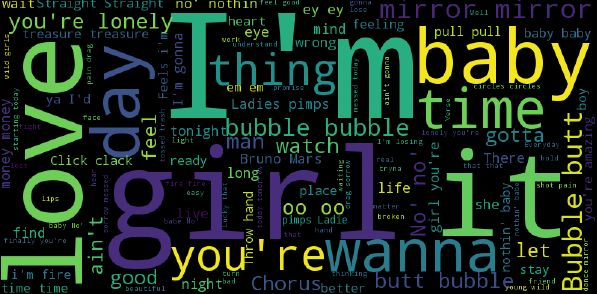
\includegraphics[width=\linewidth]{data/wordcloud}
		\caption{Wordcloud visualizing the most important terms in the lyrics of Bruno Mars. The size of the terms is related to their frequency in the lyrics. The color is only used for a more appealing visualization and does not convey any meaning.}
		\label{fig:wordcloud}
	\end{figure}
	
	To summarize pygraphml was used to export data to Gephi where visualizations involving the complete dataset were created. In addition wordclouds have been generated for the emotions and vocabularies of all individual artists. Those can be explored through the filebrowser ore more conveniently a local webserver created in flask.
	
	\section{Emotion Mining}
	\label{sec:emotionmining}
	An overview over the exact emotion mining workflow is given in this chapter. Furthermore first results are shown and discussed.
	
	The emotion mining is based on the preprocessed data. The tokenized lyrics are used and every token is looked up in an emotion lexicon for its emotional value. For our experiments, we used the \textit{NRC Emotion Lexicon} (EmoLex) \cite{emolex}.This lexicon specifies the emotional value for the eight emotions \textit{anger}, \textit{anticipation}, \textit{disgust}, \textit{fear}, \textit{joy}, \textit{sadness}, \textit{surprise}, and \textit{trust}.
	
	The emotion mining we apply to the lyrics is only rudimentary. It does not handle negations, sarcasm or complex syntactical structure. We were not able to find either an emotion lexicon that specifies the opposite emotional value for every common emotion word, or suitable work that is related to the our specific need for negated emotion words.
	
	This analysis of the tokenized songs resulted in a vector containing values for the eight emotions. These eight-dimensional emotion vector were then summed up and normalized for every artist in the dataset. For every artist the result was a vector containing information about how strong each of the eight emotions is in his songs.
	
	To calculate similarity between artists we used the cosine distance in the eight-dimensional space.
	
		\subsection{Results}
		Figure \ref{fig:emotiongraph} shows a graph of all 120 artists, where each artist is connected to a varying number of emotions. The edges have weights depending on the strength of the emotions in an artist's song. The weights are normalized between 0 and 1.
		
		The full graph of 128 nodes and 960 edges would be too ... and would not yield any useful insight. Therefore, Figure \ref{fig:emotiongraph} shows a graph that contains only those edges with sufficiently high weights. Our experiments showed that a threshold of $0.37$ yielded a balanced mixture of complexity and conciseness.
		
		\begin{figure}[htb]
			\centering
			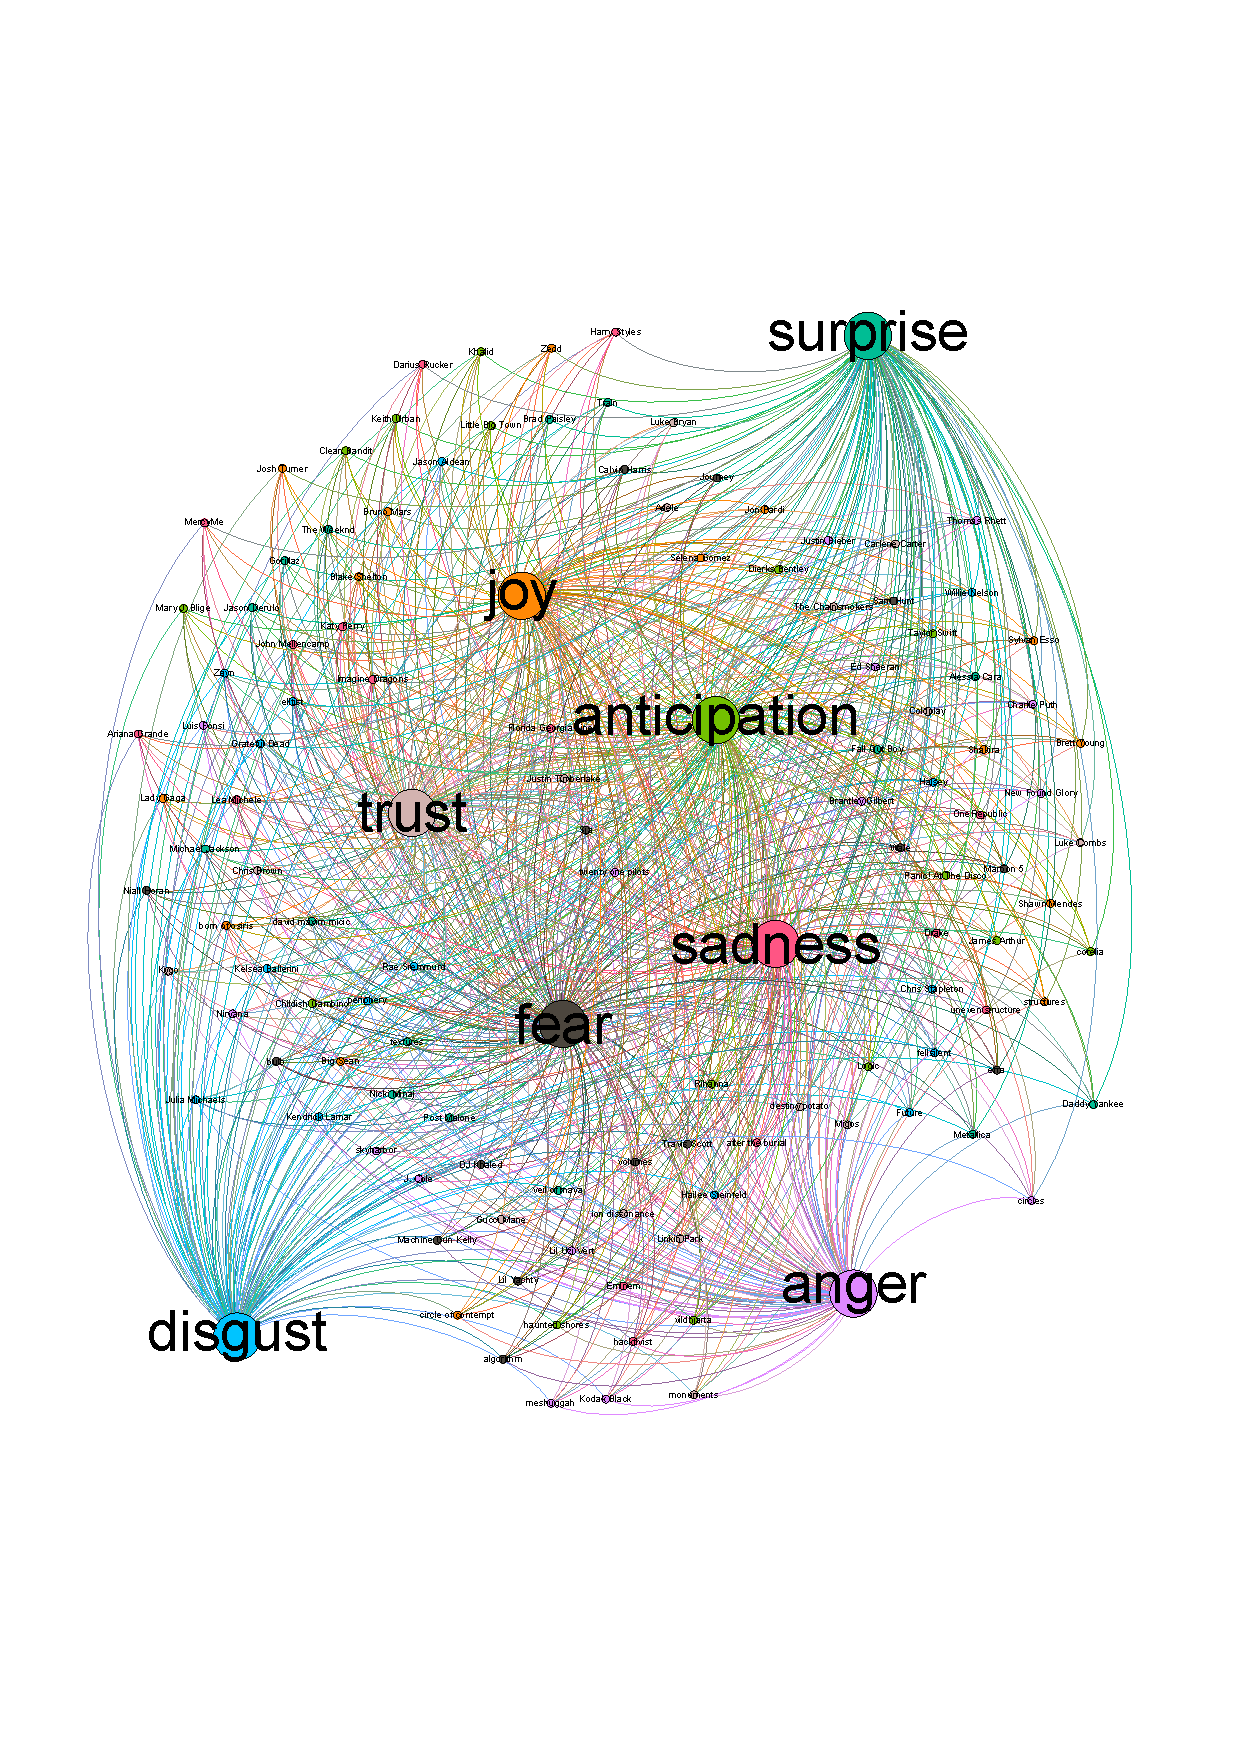
\includegraphics[trim=0mm 50mm 0mm 50mm, clip, width=\linewidth]{data/emotion_graph}
			\caption{Emotion graph with edge weight greater than $0.37$}
			\label{fig:emotiongraph}
		\end{figure}
		
		Figure \ref{fig:emotionnewmod} shows the previous graph with a newly calculated modularity score. The graph decomposes into two clusters. The first cluster is made up of the emotions \textit{anger}, \textit{fear}, \textit{sadness}, and \textit{disgust}. The second cluster consists of the emotions \textit{joy}, \textit{surprise}, \textit{trust}, and \textit{anticipation}. This partitioning seems reasonable, since it somewhat follows an intuitive understanding of positive and negative emotions.
		
		Towards these more negatively connotated emotions, there are a lot of Hip Hop, Rap, and Metal artists. In fact this kind of music is often more aggressive and ...
		Music associated with the Pop genre is closely connected to the positive emotions.
		
		\begin{figure}[htb]
			\centering
			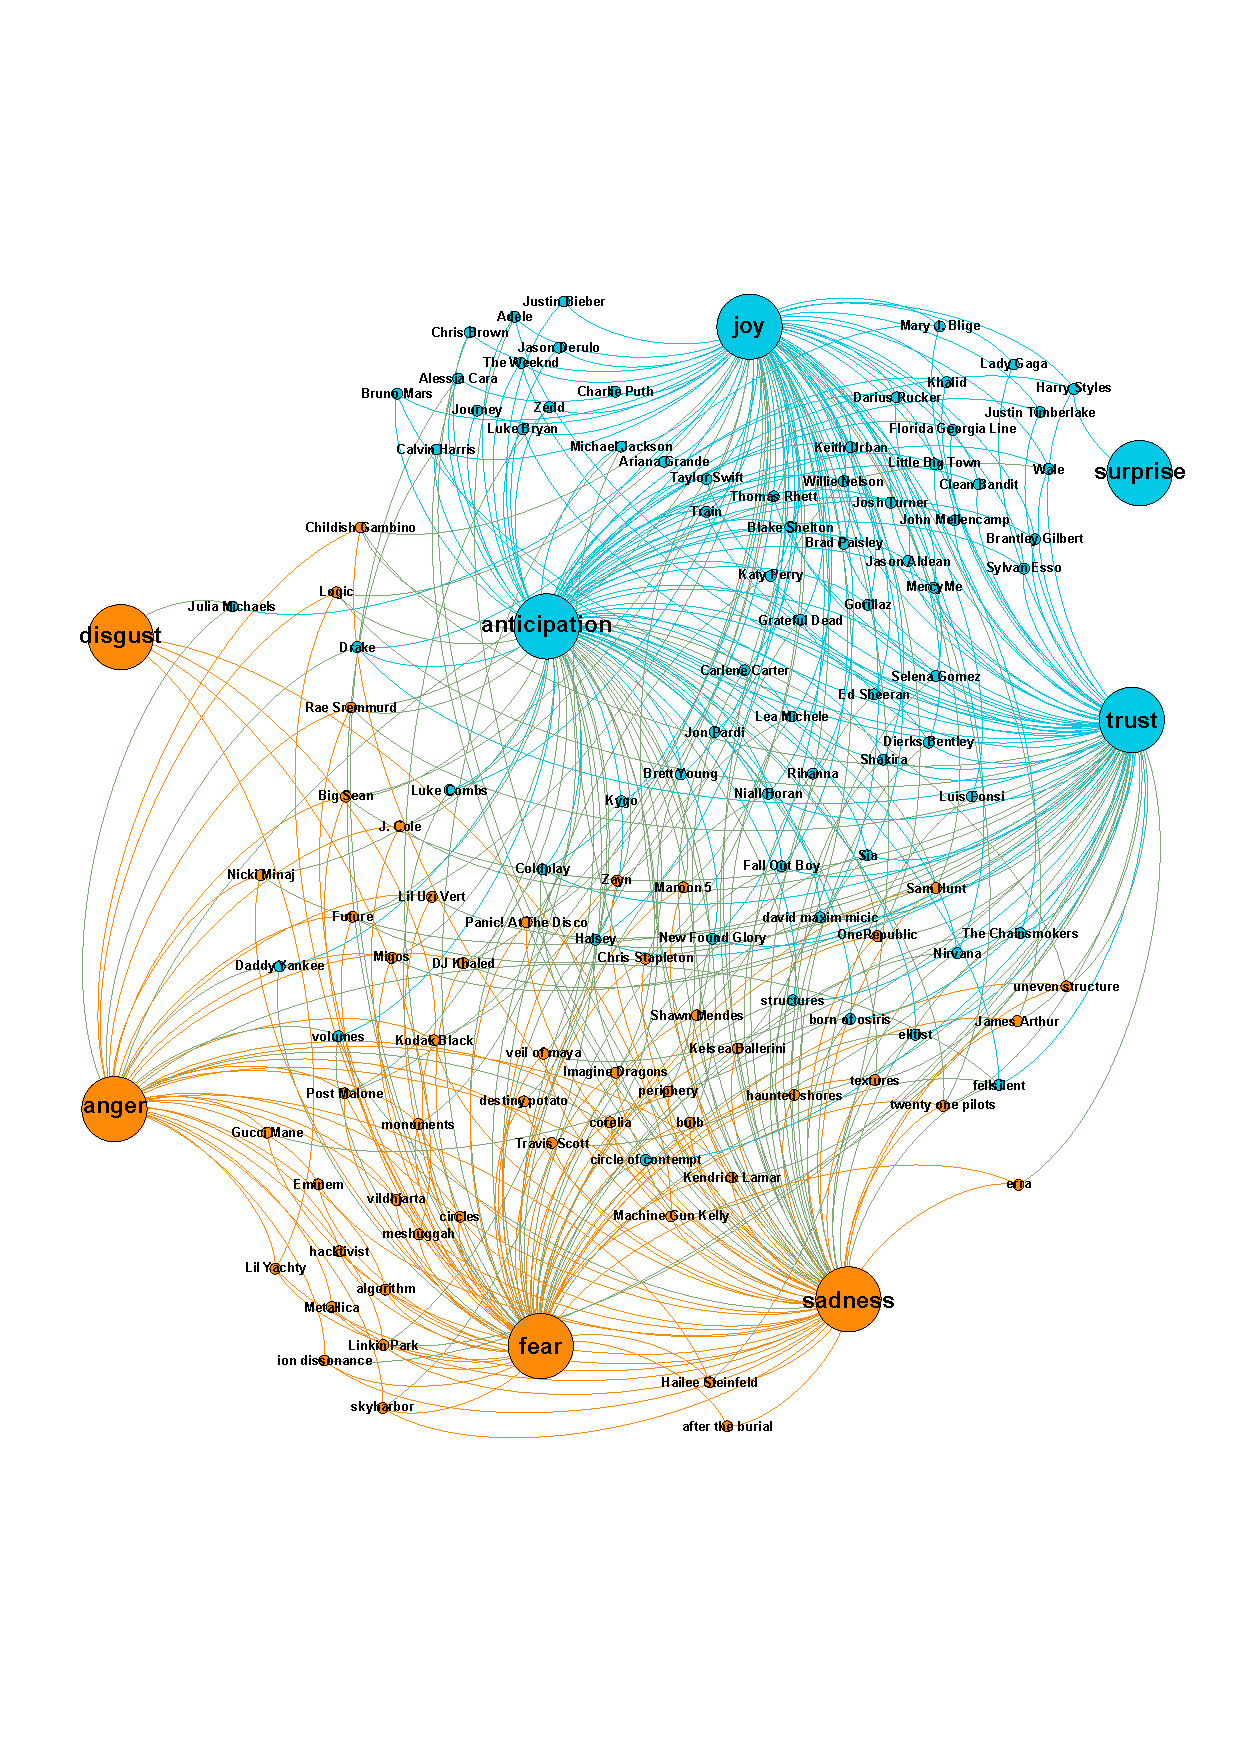
\includegraphics[trim=0mm 50mm 0mm 45mm, clip, width=\linewidth]{data/emotion_graph_new_modularity}
			\caption{Emotion graph with recalculated modularity}
			\label{fig:emotionnewmod}
		\end{figure}
		
		Figure \ref{fig:emotionsimilarity} shows the emotion similarity between individual artists. The modularity score partitions the graph into two main regions, which relate to the results shown before in Figure \ref{fig:emotionnewmod}. Pop artists are tightly clustered in one side of the graph, while Hip Hop, Rap and Metal make up the other part. Few artists whose edges have no strong enough weights are isolated from the graph.
		
		\begin{figure}[htb]
			\centering
			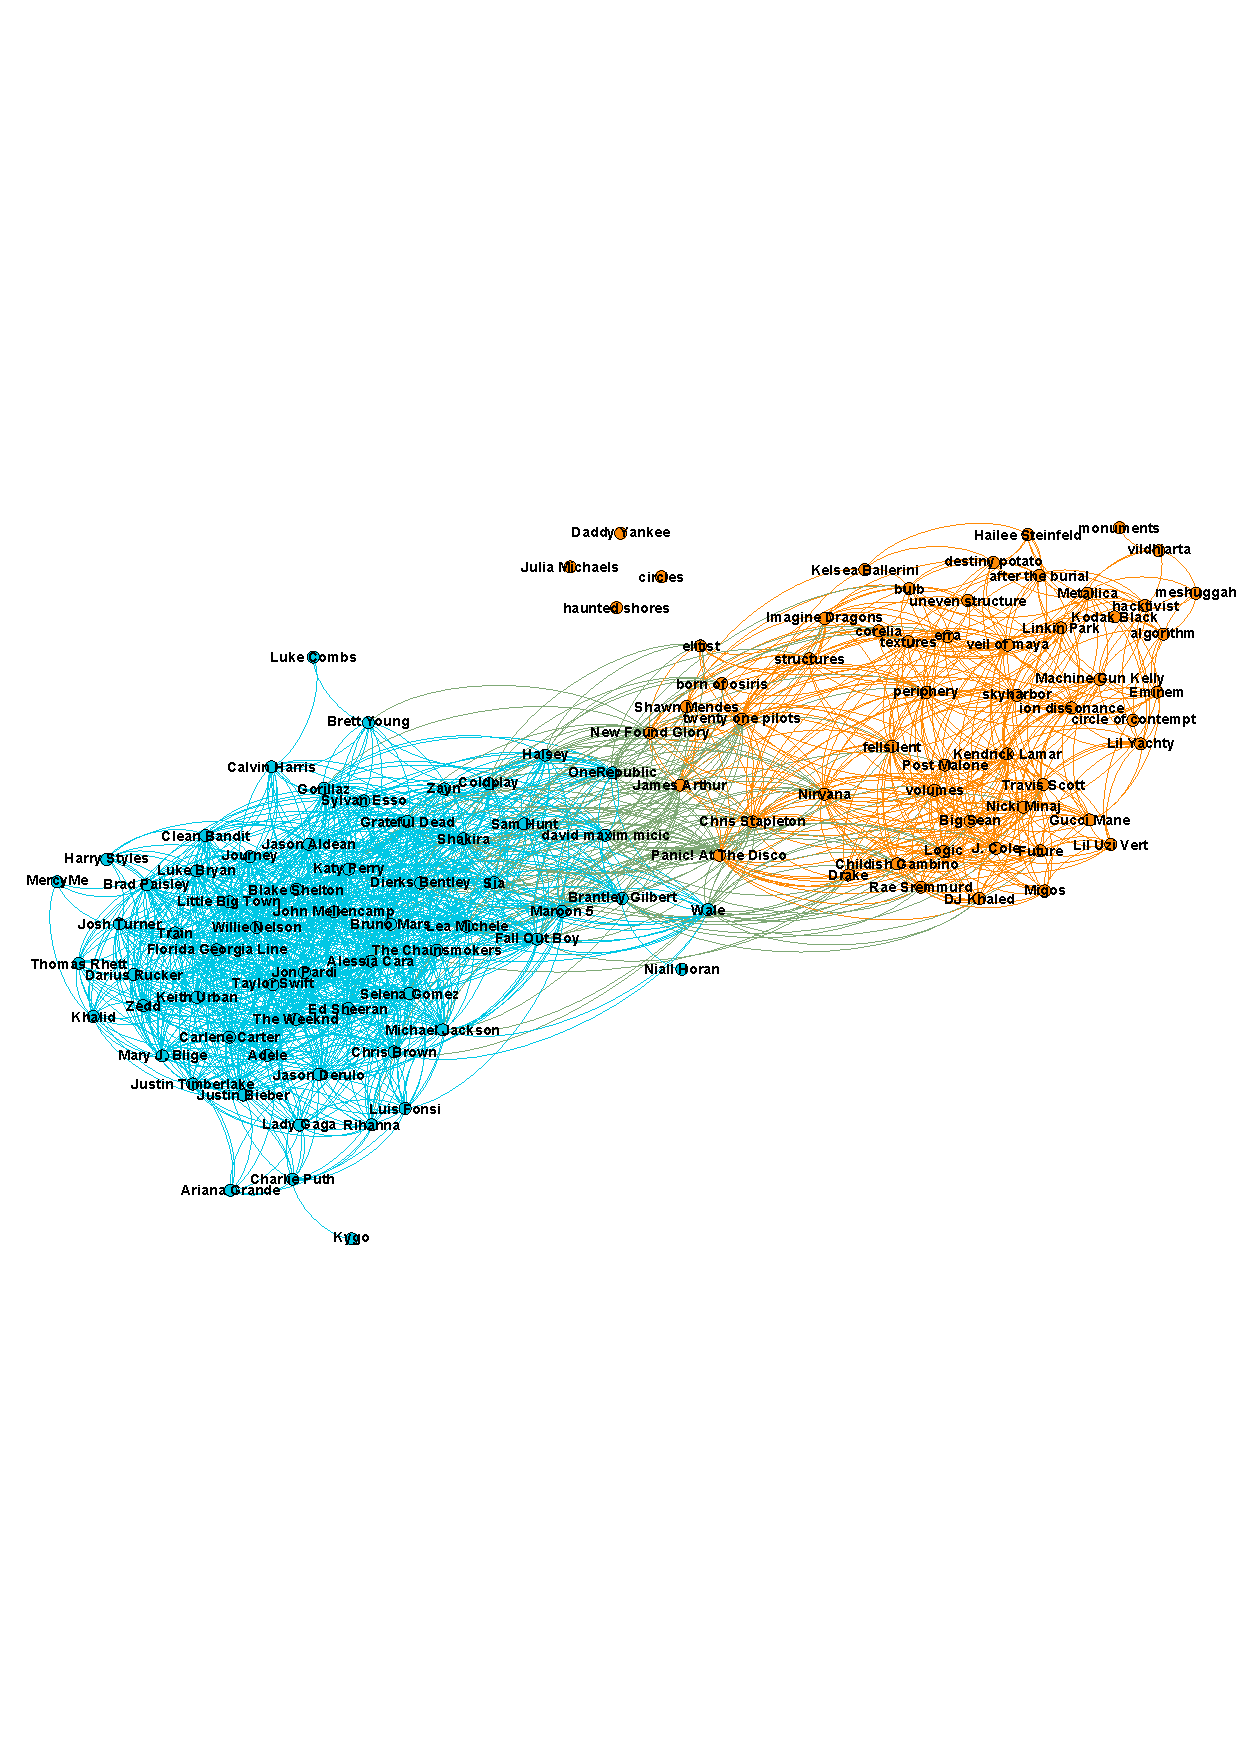
\includegraphics[trim=0mm 80mm 0mm 85mm, clip, width=0.8\linewidth]{data/emotion_similarity}
			\caption{Emotion similarity between artists greater than $0.98$}
			\label{fig:emotionsimilarity}
		\end{figure}
	
	\section{Topic Extraction}
	\label{sec:topicextraction}
	While grouping artists by emotions they express through their lyrics already provides fascinating results another part of this project was the topic based analysis of lyrics. This chapter describes the used technique and discusses the achieved results.
	
	The Non-negative Matrix Factorization (NMF) algorithm has been used to extract potential topics from the lyrics. The \textit{sklearn} Python package provides everything necessary to apply NMF to the data. In the preprocessing TF-IDF features have been calculated, which can now be used in the NMF algorithm. The NMF algorithm requires to predefine the number of expected topics and through experiments we determined ten topics to be appropriate for our dataset. 
	
	Generating more topic yielded overlap throughout the topics and creating fewer topics resulted in very packed clusters with much information contained. The amount is of course subject to the experimentalist's taste. For future work one could also experiment with hierarchical topics but we felt the topics were already very focused such that splitting them up any further would not increase the informativeness of the results.
	
		\subsection{Results}
		Similar to the results of the emotion mining before, the graph in Figure \ref{fig:topicgraph} shows all 120 artists, each of them connected to a varying number of topics, depending on the strength. All weights are again normalized between 0 and 1. The graph shows only those edges that have a weight of at least $0.32$
		
		\begin{figure}[htb]
			\centering
			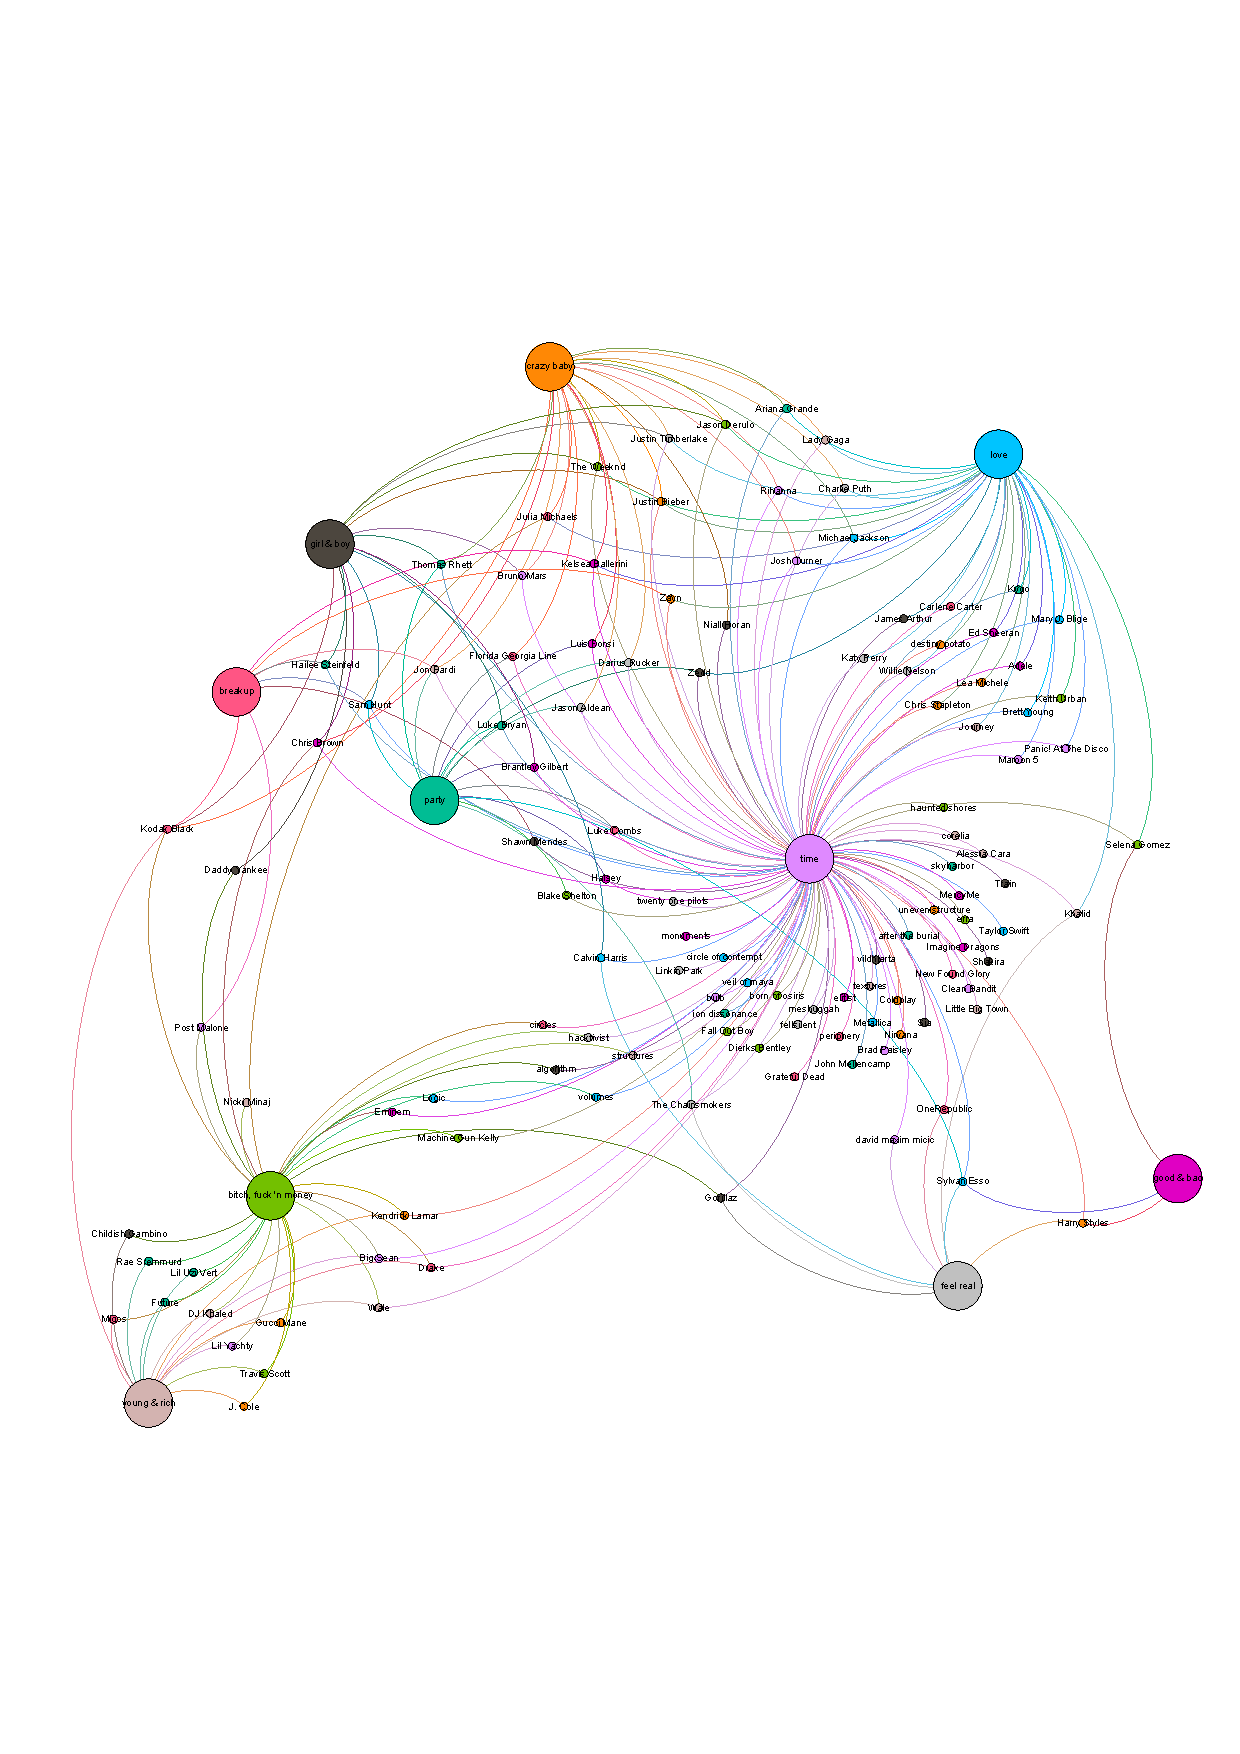
\includegraphics[trim=0mm 50mm 0mm 50mm, clip, width=\linewidth]{data/topic_graph}
			\caption{Topic graph with edge weights greater than $0.32$}
			\label{fig:topicgraph}
		\end{figure}
		
		Figure \ref{fig:topicnewmod} shows the partitioning of the graph after calculating the modularity score. The graph is partitioned into four clusters. The first one consists of the topics \textit{young \& rich}, and \textit{bitch, fuck 'n money}. The second cluster has the topics \textit{feel real} and \textit{good \& bad}. The third cluster contains the topics \textit{time} and \textit{party}. The fourth and biggest cluster is made up of the emotions \textit{breakup}, \textit{girl \& boy}, \textit{crazy baby}, and \textit{love}.
		
		%Some blabla about why this is reasonable
		
		\begin{figure}[htb]
			\centering
			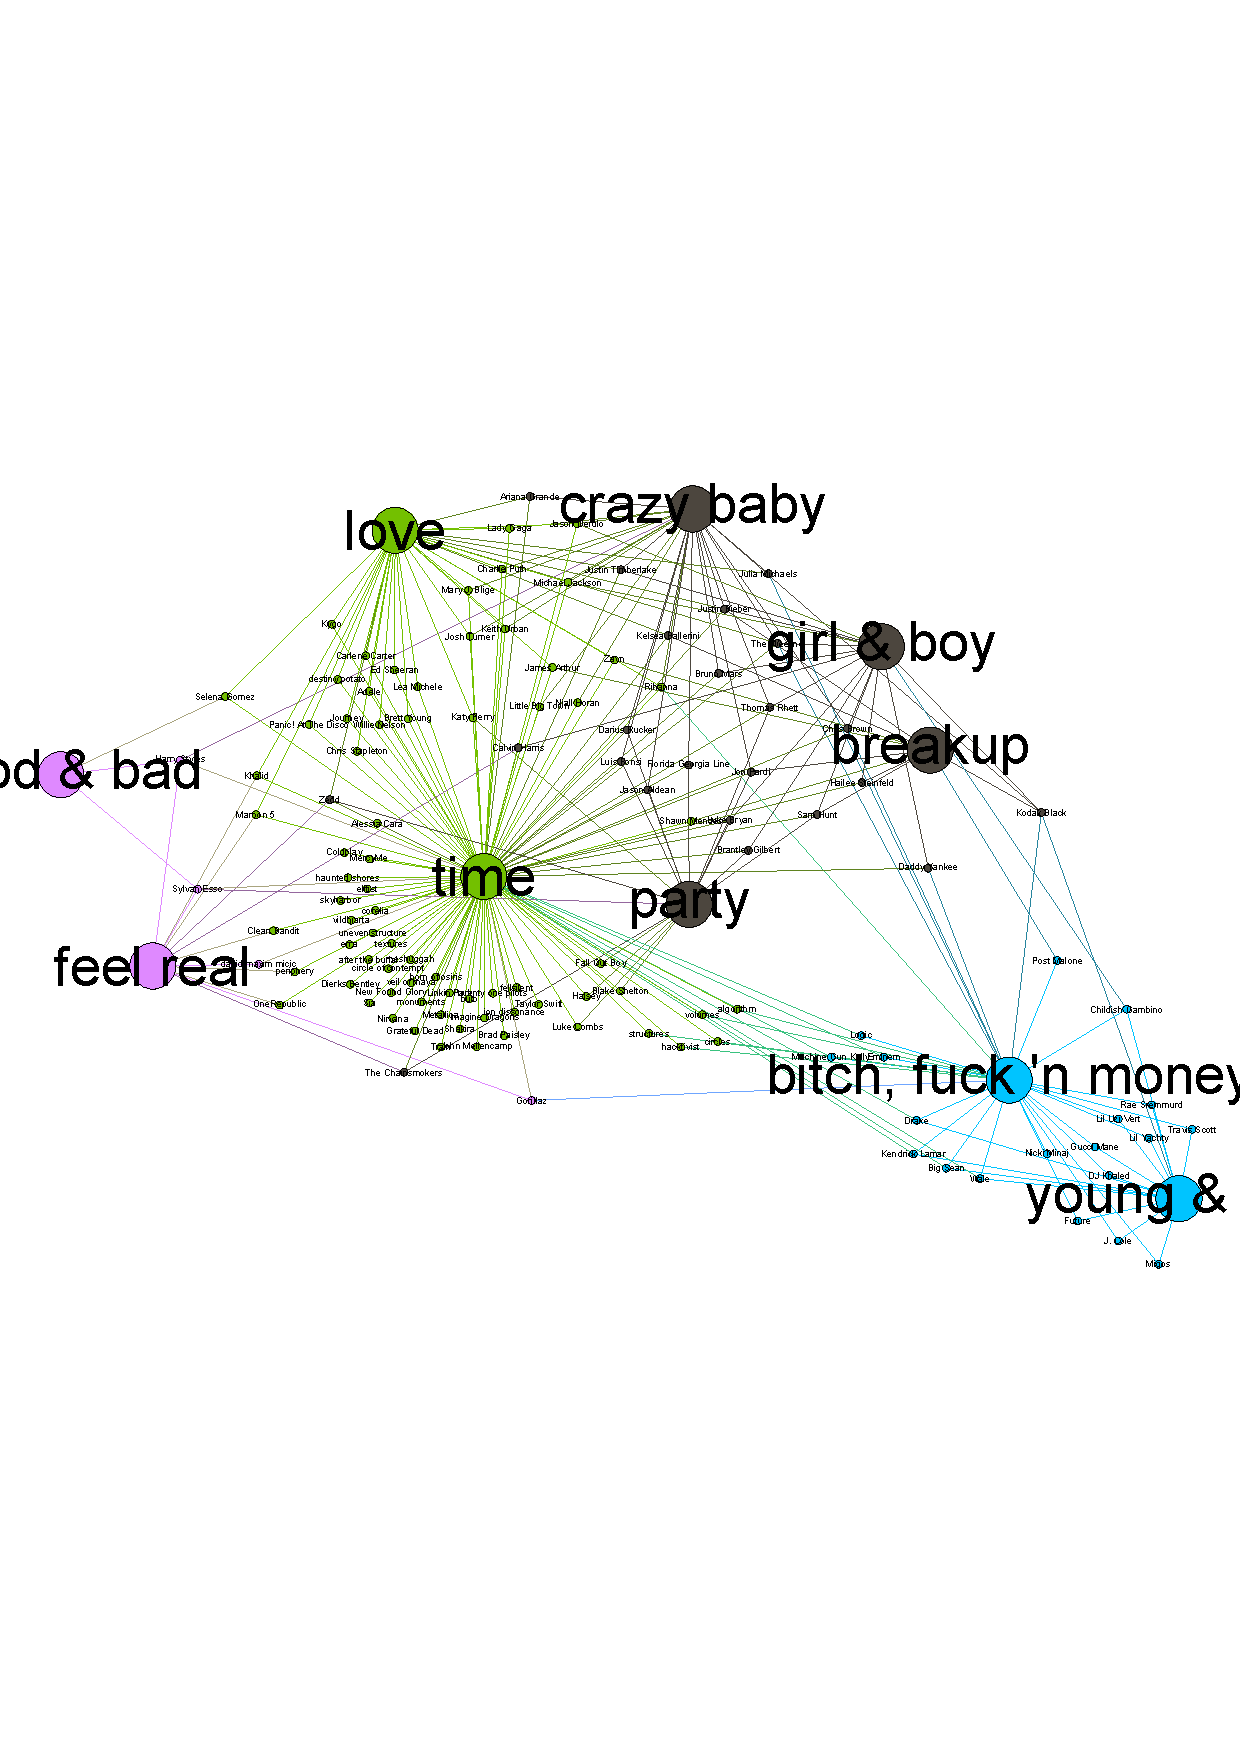
\includegraphics[trim=0mm 50mm 0mm 50mm, clip, width=\linewidth]{data/topic_graph_new_modularity}
			\caption{Topic graph with recalculated modularity}
			\label{fig:topicnewmod}
		\end{figure}
		
		Figure \ref{fig:topicsimilarity} shows the similarity of topics between artists. The modularity score partitions the graph into three components. It is interesting to see that a lot of the rappers form their own subgraph, that is only connected to the rest of the graph by the artist \textit{Daddy Yankee}\footnote{Of course, the edge weight filter is chosen such that this strongest connection between the two parts survives.}.
		
		\begin{figure}[htb]
			\centering
			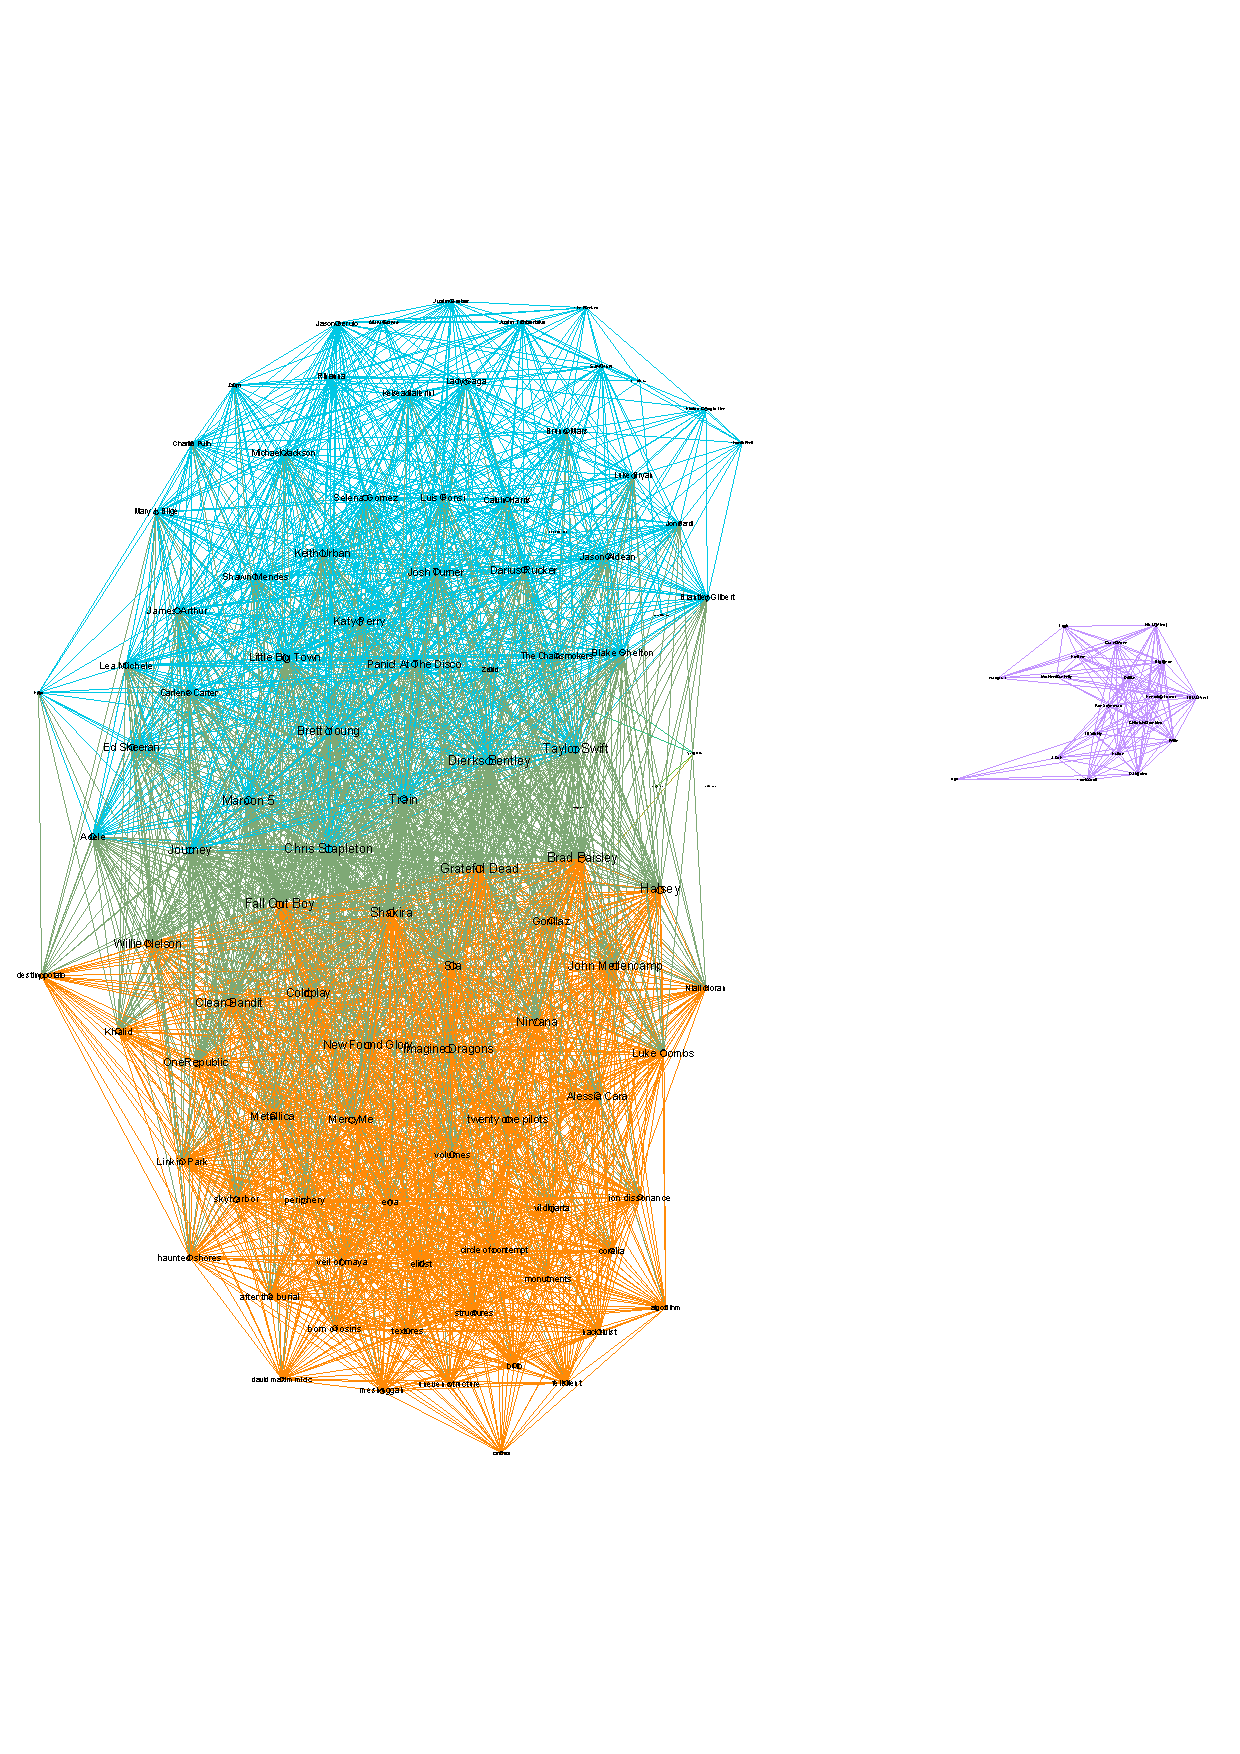
\includegraphics[trim=0mm 70mm 0mm 70mm, clip, width=\linewidth]{data/topic_similarity}
				\caption{Topic similarity between artists greater than $0.82$}
				\label{fig:topicsimilarity}
		\end{figure}
		
		\subsection{Evaluation}
		We tried to evaluate the resulting topics via held-out tests. For this, we assigned a label from $0$ to $9$ to each song depending on the highest component in its ten dimensional topic vector. We splitted the songs for each topic into a training and a test set and trained and SVM with the songs' TF-IDF features.
		
		The result of this approach...
	
	\section{Other techniques}
	\label{sec:othertechniques}
	In this section we want to mention some of the techniques we used that were neglected during the development. Some were already mentioned earlier and some have not yet been discussed at all. While we did decide not to include these techniques in our project no generality should be inferred from this as we rejected some techniques based on lack of experience, time complexity or simply the quality of the API and documentation.
	
	Part-of-Speech Tagging as well as Named Entity Extraction are techniques often used in the NLP domain. The nltk toolkit offers endpoints for both and can use different engines like the components created by the \textit{Stanford NLP Group} or can even be trained on a custom text corpus. We implemented both techniques to extract additional information from the lyrics, but non of our high-level goals (emotion mining and topic extraction) benefited from the invested effort. 
	
	While especially the NER tags can provide some intuition about the topic of a song to the user they don't actually help increase our performance in general. Only working with specific parts of speech or named entities distorts the results of emotion mining and is required in topic extraction. As we use NMF for the extraction of topics the TF-IDF values of words are used and the importance of words is already contained. NER tags could be useful if we would require information about e.g. persons or locations, but none of that yields any relevance in the context of this project.
	
	Another technique that partly suffered from the same issues was summarization. While interesting it did not really fit the scope of this project and would only obfuscate results for emotion mining and topic extraction. Furthermore, due to the complexity or simplicity of some lyrics, this could make for a whole project on it's own.
	
	During preprocessing we initially included some metrics that contained information about the lyrics readability or the complexity of the vocabulary. While the correlation between such statistics and the topics/emotions lyrics convey this was also not in the scope of this project. Furthermore the statistics could vary greatly within the songs of the same artist as they touch different styles of writing.
	
	The last technique we also applied was Rapid Automatic Keyword Extraction (RAKE). It helps, like named entities, getting some understanding about the context of a song without actually having to read the lyrics. While we used it to quickly verify our results and to verify the word clouds it does not have any benefit for the final results.
	
	To sum it up many of the techniques that are often applied, like POS and NER tagging are not required in emotion mining and topic extraction. They could even reduce the quality of the results by obfuscating the actual truths through badly handcrafted rules. The correlation of topics or emotions and the complexity of lyrics is an interesting topic, but not within the scope of this project. 
	
	% Futur Work ?

	\section{Conclusion}
	\label{sec:conclusion}
	
	\newpage
	
	\bibliography{rp}
	\bibliographystyle{apacite}
	
\end{document}